\section{Answers to Questions}

The following chapters will give answers to the questions which were raised in section 3.3. All relevant clauses and sub clauses of the standard EN 50128:2011 will be addressed and grouped in three main categories as stated in section 3.2 \FIXME{\%citation of chapter. }

\subsection{Answers to the Question}
\bigskip
\paragraph{What measures have been taken to satisfy EN 50128?}
Hereafter the applied measures will be listed according to the structure and requirements of the EN 50128:2011.

\subsubsection{Project Quality Assessment}
\paragraph{Goals, conformity and SIL [EN 50128 Section 4]}

{\itshape
Goal: allocating the safety related system functions to openETCS SW, as well as SW APIs shall be identified in the system documentation. Also the SW-SIL shall be specified here. }

\bigskip
The system in which the openETCS software will be embedded is fully defined. The Safety Integrity Level of the openETCS software is SIL 4 and it will be developed according to EN 50128:2011.

\bigskip

Assessment:
\bigskip

All the documents needed are provided by the European Railway Agency and they did already exist at the begin of the project.\\
This requirement of the standard is fulfilled.

\bigskip

\bigskip

\subsubsection{Personnel and responsibility [EN 50128 section 5.1 and 5.2]}
\itshape{Goal: Ensure that all the staff members are accountable for the software, are organized, competent and capable of exercising this responsibility.}

The document D1.3.1 Project ``\textit{Project Quality Assurance Plan}'' (QAP) has been examined.

{\bfseries
ASS512.1}


\bigskip

The openETCS project has been organizaed in seven work packages (WP1 to WP7) where each WP has its own WP-Leader and team members who shall fulfill the roles and their inde-pendency required in the EN 50128:2011. The following image shows the minimum require-ments for the independence of the assessor as well as that between the members of the pro-ject team.

 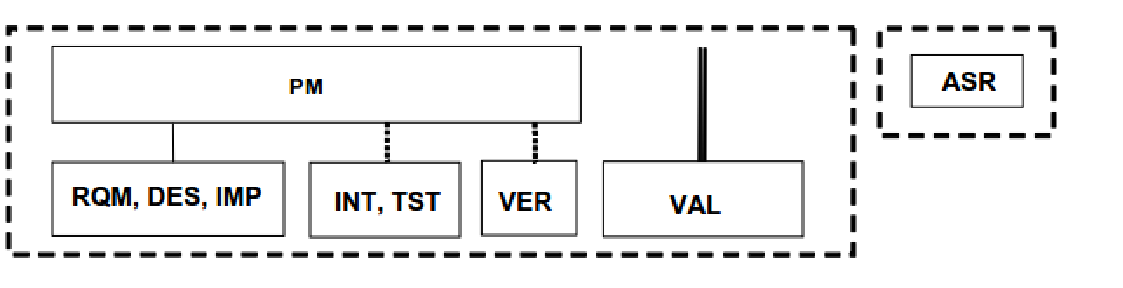
\includegraphics[width=13.626cm,height=3.493cm]{images/organizationalstructure.pdf} 

Figure 2: Preferred organizational structure for SIL 4 SW-Development

WP-Leader 1 (WPL1) is the project manager of the whole project. For the actual development three WPLs have an equivalent role to that of a project manager depicted in Figure 2 \FIXME{\%citataion of graphic}
. Other roles are distributed within the different WPs depending on their tasks and goals.


\bigskip

\begin{center}
\tablefirsthead{}
\tablehead{}
\tabletail{}
\tablelasttail{}
\begin{supertabular}{|m{5.467cm}|m{5.467cm}|m{3.467cm}|}
\hline
EN 50128:2011 Role  &
Person  &
WP (Entity) \\\hline
Project manager of all WPs  &
Mr. Dr. Hase (DB)  &
WP1 \\\hline
WPLs as Project manager  &
Mr. Cochetti (Alstom)  &
WP3\\\hline
~
 &
Mr. Behrens (DLR) &
WP4\\\hline
~
 &
Mr. Deutsch (ERSA)  &
WP5\\\hline
~
 &
Mr. Jastram (Formal Mind)  &
WP7\\\hline
\end{supertabular}
\end{center}
Table 1 Work package Leaders as project manager

\bigskip

\textbf{Assessment}:

For the targeted SIL 4 the roles were chosen appropriately within the openETCS organization. There are seven WPLs where the WPL1 is also the leader of all WPLs. The Assessors have examined the independencies of the roles within the openETCS organization and came to fol-lowing conclusions:

{}-- –	Although the validator belongs organizationally to WP4 he is an independent entity in the openETCS project and does not underlie the WPL1, WPL3, WPL5 nor WPL7.

{}-- –	The verifiers are not the same persons as the entities integrator, Tester, requirements manager, designer nor implementer

{}-- –	The independency of the rest of the entities is guaranteed according to Figure 2 \FIXME{\%citataion of graphic.}


Due to the fact that every project partner is ISO 9001 certified in addition to the many technical discussions the assessors had held with the WPLs or the many attended openETCS Scrum meetings the assessors can confirm the competences of the WPLs and their team, which are listed in the competence matrix in the QAP.
The training and qualification of the project participants is also sufficient for the tasks to be im-plemented. For example a SCADE Suite training is held for all partners using the SCADE Suite software tool in 2014.

This requirement of the standard is fulfilled.


\subsubsection{5.1.3 Life cycle and documentation [EN 50128 section 5.3]}
\textit{Goal: Organization of the software development into set phases and activities as well as registration of all the information used for the software throughout the entire life cycle of the software.}
\bigskip

The documents D1.3.1 ``Project Quality Assurance Plan''(PQAP), D2.3a ``Definition of the openETCS Development Process'' and D2.3b ``Scrum Process in the openETCS Project'' have been assessed.

\textbf{Assessment}:
\bigskip

A life cycle model that is based on the suggested model of the standard is referenced in the quality assurance plan. In document D2.3a the process goals and activities of the model are described as well as the documents and artifacts to be created in each phase of the develop-ment life cycle. The documents (deliverables) are created with the open source tool LaTeX.

For the targeted SIL of the SW development in the openETCS project an appropriate and de-tailed life cycle model was chosen, the V-Model. Each individual phase of the V-Model was completely defined with clear inputs, outputs, responsible EN 50128 roles and activities to be done (see Figure 3) \FIXME{\%citataion of graphic.}

\bigskip

\FIXME{\% including graphic openETCS Development Lifecycle Figure 3 in the word document}

\bigskip

However, in D2.3a it is stated that the phases of the development life cycle “may overlap in time” and therefore they will not be processed in a clear consecutive order. This is due to the agile SW development approach applied by Scrum. It is described in D2.3b, where these life cycle phases with their complex tasks are broken down into increments and then executed in short time frames called sprints.

\bigskip

\textbf{Assessment}:

The approach of choosing the V-Model for defining each phase of the life cycle and then im-plementing the Scrum methodology for the SW development does totally comply with all the clauses and sub clauses of § 5.3.
This requirement of the standard is fulfilled. 



\subsubsection{5.1.4 Software quality assurance [EN 50128 section 6.5]*}

\tiny{(*): other EN 5018 parts to be examined in \textit{sections 7.3.4.25 to 7.3.4.27 related to coding standards.} }

\textit{Goal: Identification, monitoring and controlling of all technical and management activities that are necessary in order
to ensure that the software attains the required quality. This is necessary to guarantee the required qualitative defense against systematic faults and to ensure that an audit can be set up to make it possible to efficiently take verification and validation measures.}

\bigskip
The plans for the quality assurance procedure were created at the beginning of the project. Due to the agile process, these plans have been updated iteratively. They shall demonstrate in detail how the quality assurance of the software can be guaranteed during the entire develop-ment life cycle. A quality assurance plan describes the methodology and measures in each project phase, a verification and validation plan describes the verification and testing activities, a maintenance plan describes the quality assurance process for maintenance and modification activities.
\bigskip

\textbf{Assessment}:

\bigskip

For the targeted SIL an appropriate amount of techniques and measures shall be chosen. The SCADE Suite development tool, in which the openETCS on-board unit SW was developed, covers great amount of them. However, in the quality assurance plan it should be stated which technique or measures for the SIL 4 SW development was covered and if not a justification for not applying a technique or measure, which is labeled with “M” (Mandatory) or “HR” (Highly Recommended) should be noted. And if more than one technique/measure was applied the approved combination of these techniques in the standard shall be followed.

\bigskip

\paragraph{Table A1 Lifecycle Issues and Documentation in the EN 50128:2011:}
Already covered in section 5.1.1.3

\paragraph{Table A2 Software Requirements Specification in the EN 50128:2011:}
 
The application of the techniques and measures of this table are well documented in D1.3.1.
This requirement of the standard is fulfilled.

\paragraph{Table A3 in the EN 50128:2011: }

There are more than one technique or measure, which were applied and documented in D1.3.1. The requirement for an approved combination for SIL 4 in Table A2 from the standard was not considered.
This requirement of the standard is not fulfilled.


\paragraph{Table A4 in the EN 50128:2011:}
 
The application of the techniques and measures of this table are well documented in D1.3.1. The non-application of techniques or measures are justified.
Recommendation: The chosen combination of those techniques shall be clearly stated after each table for SIL 4 development (e.g Combination of 4 5, 6, 8 and one of 1 or 2).

This requirement of the standard is fulfilled.

\paragraph{Table A5 in the EN 50128:2011:}

The application of the techniques and measures of this table are well documented in D1.3.1. The non-application of techniques or measures are justified.
Recommendation: The chosen combination of those techniques shall be clearly stated after each table for SIL 4 development (e.g the combination of 3, 5, 7, 8 and one of 1, 2 or 6).

This requirement of the standard is fulfilled.

\paragraph{Table A6 in the EN 50128:2011:}

The application of the techniques and measures of this table are well documented in D1.3.1. The non-application of techniques or measures are justified.
This requirement of the standard is fulfilled.

\paragraph{Table A7 in the EN 50128:2011:}
The application of the techniques and measures of this table are well documented in D1.3.1.

This requirement of the standard is fulfilled.

\paragraph{Table A8 in the EN 50128:2011:}
The application of the techniques and measures of this table are well documented in D1.3.1. The non-application of techniques or measures are justified.

This requirement of the standard is fulfilled.

Recommendation: It should be reviewed if these statements in Table A8 are accurate to the activities of the project.

\paragraph{Table A9 in the EN 50128:2011:}
The application of the techniques and measures of this table are well documented in D1.3.1. The non-application of techniques or measures are justified.

This requirement of the standard is fulfilled.

\paragraph{Table A10 in the EN 50128:2011:}
The application of the techniques and measures of this table are well documented in D1.3.1. The non-application of techniques or measures are justified.

This requirement of the standard is fulfilled.

\paragraph{Table A11 in the EN 50128:2011:}
The application of the techniques and measures of this table are well documented in D1.3.1. The non-application of techniques or measures are justified.

This requirement of the standard is fulfilled.

\paragraph{Table A12 in the EN 50128:2011:}
Following techniques/measures in table A12 of the standard are not documented:

\begin{enumerate}
\item	Coding Standard (M)
\item	Coding Style Guide (HR)
\item	No Dynamic Objects (HR)
\item	No Dynamic Variables (HR)
\item	Limited Use of Pointers (R)
\item	Limited Use of Recursion (HR)
\item	No Unconditional Jumps (HR)
\item	Limited size and complexity of Functions, Subroutines and Methods (HR)
\item	Entry/Exit Point strategy for Functions, Subroutines and Methods (HR)
\item	Limited number of subroutine parameters (R)
\end{enumerate}

This requirement of the standard is not fulfilled.

\paragraph{Table A13 in the EN 50128:2011:}
Following techniques/measures in table A12 of the standard are not documented:

\begin{enumerate}
\item	Test Case Execution from Boundary Value Analysis (HR)
\item	Test Case Execution from Error Guessing (R)
\item	Test Case Execution from Error Seeding (R)
\item	Performance Modelling (HR)
\item	Equivalence Classes and Input Partition Testing (HR)
\item	Structure-Based Testing (HR)
\end{enumerate}

This requirement of the standard is not fulfilled.

\paragraph{Table A14 in the EN 50128:2011:}
Following techniques/measures in table A12 of the standard are not documented:
\begin{enumerate}
\item	Test Case Execution from Cause Consequence Diagrams (R)
\item	Prototyping/Animation (R)
\item	Boundary Value Analysis (HR)
\item	Equivalence Classes and Input Partition Testing (HR)
\item	Process Simulation (R)
\end{enumerate}

This requirement of the standard is not fulfilled.

\paragraph{Table A17 in the EN 50128:2011:}
Following techniques/measures in table A12 of the standard are not documented:
\begin{enumerate}	
\item	Data Modelling (HR)
\item	Data Flow Diagrams (HR)
\item	Control Flow Diagrams (HR)
\item	Finite State Machines or State Transition Diagrams (HR)
\item	Time Petri Nets (HR)
\item	Decision/Truth Tables (HR)
\item	Formal Methods (HR)
\item	Performance Modelling (HR)
\item	Prototyping/Animation (HR)
\item	Structure Diagrams (HR)
\item	Sequence Diagrams (HR)
\end{enumerate}
 
This requirement of the standard is not fulfilled.

\paragraph{Table A18 in the EN 50128:2011:}
Following techniques/measures in table A12 of the standard are not documented:

\begin{enumerate}
\item	Avalanche/Stress Testing (HR)
\item	Response Timing and Memory Constraints (HR)
\item	Performance Requirements (HR)
\end{enumerate}

This requirement of the standard is not fulfilled.

\paragraph{Table A19 in the EN 50128:2011:}
Following techniques/measures in table A12 of the standard are not documented:

\begin{enumerate}
\item 	Boundary Value Analysis (HR)
\item 	Checklists (R)
\item 	Control Flow Analysis (HR)
\item 	Data Flow Analysis (HR)
\item 	Error Guessing (R)
\item 	Walkthroughs/Design Reviews (HR)
\end{enumerate}

This requirement of the standard is not fulfilled.

\paragraph{Table A.20 in the EN 50128:2011:}
Following techniques/measures in table A12 of the standard are not documented:
\begin{enumerate}
\item	Information Hiding (-)
\item	Information Encapsulation (HR)
\item	Parameter Number Limit (R)
\item	Fully Defined Interface (M)
\end{enumerate}

This requirement of the standard is not fulfilled.

\paragraph{Table A.21 in the EN 50128:2011:}
Following techniques/measures in table A12 of the standard are not documented:

\begin{enumerate}	
\item	Statement (HR)
\item	Branch (HR)
\item	Compound Condition (HR)
\item	Data flow (HR)
\item	Path (HR)
\end{enumerate}

This requirement of the standard is not fulfilled.

\paragraph{Table A.22 in the EN 50128:2011:}
Not applicable.

\paragraph{Table A.23 in the EN 50128:2011:}
Not applicable.


\paragraph{Table A1 - A23: Summary}

\textbf{Assessment:}

Not all documentations of the tables are sufficiently done and not all tables were considered and justified which is to be improved.
This requirement of the standard is therefore \textit{partially fulfilled}.


\subsubsection{Changes and change management [EN 50128 sect. 6.6]}
\textit{Goal: Ensure that the software functions as required and that the software safety requirement and reliability is retained upon modification of the software.}

The provided deliverables of the project have been examined. Not all documented activities of this requirement of the standard have been done due to the Project Quality Assurance Plan. 
\bigskip
This activity was not done in the openETCS project.
\textbf{Assessment:}
\bigskip
A change management process was defined but in some cases are not implemented.
This requirement of the standard is therefore \textit{partially fulfilled}.
\bigskip

\subsection{V\&V Assessment}

\bigskip

\subsubsection{Software test [EN 50128 sect. 6.1]*}
\textit{(*): other EN 5018 parts to be examined here = section 7.3.4.33 (software component test specification) and sections 7.3.4.29 to 7.3.4.40 (software integration and software/hardware integration specifications)
The goal of the software test is to check the behavior or performance of the software.}

\bigskip
This activity have not been done in the project.
\bigskip

\textbf{Assessment:}
\bigskip
This requirement of the standard is not fulfilled.
\bigskip

\subsubsection{Software verification [EN 50128 sect.6.2]*}
\textit{*): other EN 50128 parts to be examined here = sections 7.3.4.41 to 7.3.4.43 (software architecture and design verification).
The goal of the software verification is the investigation and evaluation based on demonstrating that the results of a certain development phase are sufficient.}
\bigskip
This activity have not been done in the project.
\bigskip

\textbf{Assessment:}
\bigskip
This requirement of the standard is not fulfilled.
\bigskip

\subsubsection]{5.2.3 Software validation [EN 50128 sect. 6.3]}
\textit{The goal of the software validation is to demonstrate that the processes and output variables of the software comply with the set SIL, satisfy the software requirements and are suitable for the intended application. The main validation activities consist of analysis and/or testing and evaluation of the safety criticality of all the faults and deficiencies.}

\bigskip
This activity have not been done in the project.
\bigskip

\textbf{Assessment:}
\bigskip
This requirement of the standard is not fulfilled.
\bigskip

\subsubsection{Software implementation and test [EN 50128 sect. 7.5]}
\textit{Goal: Creation of software that is analyzable, testable, verifiable and repairable. This phase also covers component tests.}

\bigskip
\FIXME{\%please check enumeration of the ASS524.1. or may be we can delete that structure}
We have examined the document: D4.2.2 “Preliminary Validation and Verification Report on
Implementation/Code”.
Because the document is not the final one (the project is following a SCRUM process), the missing parts are not highlighted in the assessment (for example the formal verifications are still incomplete and it is not verified that OpenETCS decoder calls the Bitwalker software only according to its specification).

{\bfseries ASS524.1}

7.5.4.1 The Software Source Code shall be written under the responsibility of the implementer on the basis of the Software Component Design Specification. Requirements from 7.5.4.2 to 7.5.4.4 refer to the software source code.
This EN requirement is not fulfilled because the Software Component Design Specification was not available (p 17 of D4.2.2 it is written “In a first step, we had to inspect the source code and derive from it an informal specification. This informal specification is to be understood as a re-quirements document for the bitwalker functions as it should have been available to both the programmer and the verifier in advance”.

{\bfseries ASS524.2}

7.5.4.5 A Software Component Test Report shall be written, under the responsibility of the Tester, on the basis of the Software Component Test Specification and the Software Source Code.
This EN requirement is not fulfilled because there is no Software Component Test Specifica-tion.

{\bfseries ASS524.3}

7.5.4.8 A Software Source Code Verification Report shall be written, under the responsibility of the verifier, on the basis of the Software Component Design Specification, the Software Component Test Specification and the Software Source Code.
This EN requirement cannot be fulfilled because both “Software Component Test Specification” and “Software Component Design Specification” are missing.

{\bfseries ASS524.4}

EN requirement 7.5.4.10 is not covered:
\begin{itemize}
\item	“a) the adequacy of the Software Source Code as a implementation of the Software Component Design Specification” is not covered. .P17 of D4.2.2 It is said that “the re-quirements document for the bitwalker functions should have been available to both the programmer and the verifier” (they have been replaced by informal specifications).
\item	“b) the correct use of the chosen techniques and measures from Table A.4 as a set sat-isfying 4.8 and 4.9”. This is fulfilled but not justified in D4.2.2.
\item	“c) determining the correct application of the coding standards” could be fulfilled but the coding standards have not been defined for the project.
\item	“d) the Software Source Code meets the general requirements for … traceability (6.5.4.14 to 6.5.4.17)…” is not fulfilled. Traceability aspects are not addressed in D4.2.2. 
\item	“e) the adequacy of the Software Component Test Report as a record of the tests car-ried out in accordance with the Software Component Test Specification” is not fulfilled because there is no Software Component Test Specification.
\end{itemize}

{\bfseries ASS524.5}

P24 of D.4.2.2 says “we assume that the C-types unsigned int and int, which are used in the implementation to represent indices, counting and error codes, have a width of 32 bits. We point this out here because we conducted the verification on a platform with these characteris-tics.
This means that the proof validity is limited to 32 bits hardware. What happens for 16 bits?

{\bfseries ASS524.6}

P30 of D4.2.2 says “Of course, rewriting the implementation while verifying it may appear odd. Ideally, the verification tool should take the code as it is”.
This is indeed a big problem!

{\bfseries ASS524.7}

Frama.C used for formal proof and the associated provers should be T3 class tools. Is it the case?

\bigskip

\textbf{Assessment:}
\bigskip
This requirement of the standard is therefore \textit{partially fulfilled}.
\bigskip


\subsubsection{Software integration [EN 50128 sect. 7.6]}
\textit{Goal: Execution of the software integration and software/hardware integration. Demonstration that the software and the hardware properly work together to perform their intended functions.}

\bigskip

This activity is out of scope.

\bigskip

\subsection{Safety Activities Assessment}

\bigskip

\subsubsection{Software assessment [EN 50128 sect. 6.4]}
\textit{Goal: Evaluation of the process of the life cycle and the products arising from it allow the conclusion that the software exhibits the set SIL 1 to 4 and is suitable for it intended use.}

\bigskip
\FIXME{\%citation of references table}
The procedure of the assessment is described in the Assessment Plan document D4.5.1. The documents necessary for an assessment as per EN 50128 are listed in tableXXX (Table of openETCS documents mapped to the required Documents of EN 50128). Due to the SCRUM process not all documents were thoroughly examined and verified.

\bigskip

\textbf{Assessment}:
\bigskip
This requirement of the standard is fullfiled.
\bigskip

\subsubsection{Supporting tools and languages [EN 50128 sect. 6.7]}
\textit{Goal: Software tools must be appropriately selected for the software development process, the tools should be able to work together, the use of tools in classes T2 and T3 must be justified and for T3 proof of suitability must be present.}

\bigskip
The software development Tool was SCADE Suite and SCADE System. These are categorized as class T3 Tools and the generated code is SIL 4 certified. This was not the case for other used tools (e.g. open source tools) and they need to be assessed first.

\bigskip

\textbf{Assessment}:

\bigskip

\subsubsection{Software requirement [EN 50128 sect. 7.2]}
\textit{Goal: Description of a complete set of requirements for the software that satisfies all the system and safety requirements and provides an extensive set of documents for each later phase.}

\bigskip
This activity has not been done in the project.

\bigskip

\textbf{Assessment}:

\bigskip
This requirement of the standard is not fulfilled.
\bigskip

\subsubsection{Software architecture and design [EN 50128 sect. 7.3]} \FIXME{\%checking the format of this chapter compared to word document}
\textit{Goal: Development of a software architecture. Identify and evaluate what the interaction between hardware and software means for safety. Selection of a design process. Design of the software of a defined SIL. Ensure that the resulting system and its software can easily be tested from the outset.}

We have examined the document: D3.5.3 ``openETCS Architecture and Design Specification''.

Notice that the section 7.3 of EN 50128 covers not only architecture, interface and design specifications but also test
specification for software component test, software integration and software/hardware integration. These elements are
not covered by D3.5.3. So section 7.3.4.33 and sections 7.3.4.29 to 7.3.4.40 have been transferred to \& 5.2.1 of this
document. For the same reason, sections 7.3.4.41 to 7.3.4.43 dealing with verification have been transferred to \& 5.2.2
of this document, and sections 7.3.4.25 to 7.3.4.27 related to coding standards have been transferred to \& 5.1.4 of
this document.

{\bfseries ASS534.1}

Considering the safety aspects we have some doubt about the robustness of the proposed design. Theoretically the
following fields ``Behaviour when value is at boundary / Behaviour for values out of valid range / Behaviour when value
is erroneous, absent or unwanted'', given for all inputs should explain which safety mechanisms have been implemented
and how they work . Numerous remarks can be done on these fields:

{\textbullet} Sometimes the behavior in case of ``erroneous data'' is considered as identical to the behavior in case of
``data at the boundary'' which is not acceptable (see for example 5.2.2.1.3 ActualOdometry; 5.2.2.1.11
inSupervisingRbcId {\dots}).

{\textbullet} Sometimes the behavior in case of ``erroneous data'' could result in a hazard but no safety mechanism is
proposed (see for example 5.2.2.1.13 q\_nvlocacc; 5.3.2.1.2 Status\_MA\_FS\_SR\_OS\_LS\_SH\_from\_MA\_L2\_Management;
5.3.2.1.8 statusValid\_Position\_from\_Position\_Calculation {\dots}).

{\textbullet} A majority of these fields indicates ``n/a'' and that seems very curious for a SIL4 software. These n/a
should be justified (For example, the input ``5.9.2.1.19 SafetyCriticalFailure'' is considered has having no effect
when it is absent or erroneous which is very curious considering the name of the data).


\bigskip

{\bfseries
ASS534.2}

Requirement 7.3.4.5 of the EN 50128 is: ``The Software Architecture Specification shall identify, \textbf{analyse and
detail the significance} of all hardware/software interactions''. This requirement is not fulfilled.


\bigskip

{\bfseries
ASS534.3}

Requirement 7.3.4.6 b) of the EN 50128 is: ``Software components shall be clearly identified and \textbf{independently
versioned inside the configuration management system}{}''. This requirement is not fulfilled.


\bigskip

{\bfseries
ASS534.4}

The following EN 50128 requirements are not fulfilled:

{\textbullet} 7.3.4.10 The Software Architecture Specification shall \textbf{describe the strategy for the software
development} to the extent required by the software safety integrity level. 

{\textbullet} 7.3.4.11 \textbf{Measures for handling faults} shall be included in the Software Architecture
Specification in order to achieve the balance between the fault avoidance and fault handling strategies.


\bigskip

{\bfseries
ASS534.5}

The Software Interface Specification (see requirements 7.3.4.18 and 7.3.4.19 of EN 50128) is missing. The description of
interface data given in D3.5.3 is incomplete [a) pre/post conditions; f) allocated memory, f) and h) synchronization
mechanisms are missing].


\bigskip

{\bfseries
ASS534.6}

The description given in the software design part does address neither the main algorithms and sequencing or concurrency
aspects, nor the error reporting mechanisms (see f) and g) of requirement 7.3.4.23 of EN 50128 and b3) and b4) of
requirement 7.3.4.28 of EN 50128. 


\bigskip

\textbf{Assessment}:

Design Specification is incomplete (Scrum process) but numerous requirements of the CENELEC standard are not fulfilled
and will not be if the content of the document is not modified. 

Notwithstanding these previous remarks, a major remark is that safety aspects are not well addressed in this design.

\subsubsection{Software components design [EN 50128sect. 7.4]}
\textit{Goal: development of a software component design and software component test specifications, with which the requirements of the software design specifications are satisfied to the extent required by the SIL.}

\bigskip
For this activity is the documentation is missing.

\bigskip

\textbf{Assessment}:
\bigskip
This requirement of the standard is not fulfilled.

\bigskip

\subsubsection{Overall software test [EN 50128 sect. 7.7]}
\textit{Analysis and test of the integrated SW and HW in order to ensure accordance with the software requirement specifications, especially the functional and safety aspects as per the SIL.}


\bigskip

This section is out of scope.
\bigskip

\subsubsection{Application data or algorithms -- systems configured by application data or algorithms [EN 50128 sect. 8]}

\bigskip

This section is out of scope.
\bigskip

\subsubsection{Deployment of the software [EN 50128 sect. 9.1]}
\textit{Goal: Ensure that the software works as intended, adheres to the required SIL and reliability when it is deployed in the final environment of application}


\bigskip

This section is out of scope.
\bigskip

\subsubsection{Maintenance of the software [EN 50128 sect. 9.2]}
Goal: Verification that the software functions as required and the obligatory SIL and reliability are maintained if
corrections, extensions or adjustments are performed on the software.
\bigskip

\bigskip

This section is out of scope.
\bigskip

\subsection{Answer to the question: Are the measures taken for satisfying EN 50128 SIL 4 sufficient?}
\bigskip
The techniques and measures from table A.1 to A.10 with the detailed tables A.12 to A.23 ap-plied for software development were all evaluated in section 5.1.
\newline
\newline

By applying the methods and processes of the standard EN 50128:2011 this question has been partially satisfied. 
\bigskip

\subsection{Answer to the question: Is the agile development practiced in the openETCS project complying with requirements of the EN 50128:2011?}

\bigskip
Generally the CENELEC standard EN 50128:2011 doesn’t stipulate a specific development process model. It solely makes recommendation for applying a development model that is able to fulfill all the EN 50128 requirements. We consider that it is the case for the Agile model provided it is accompanied with sound configuration management and change management processes.
\newline
\newline
Based on this fact the SCRUM methodology was implemented. This agile framework has allowed continuous refinements and improvements throughout the whole openETCS software development process. The roles and activities of the WPL and WP members have practiced in this agile framework without being in conflict with the requirements of the EN 50128:2011.
\newline
\newline
The assessors find no contradiction of applying the agile SCRUM-Methodology in openETCS project with the CENELEC standard EN 50128:2011.
\bigskip

\FIXME{\%include graphic Figure 4 Scrum methodology from the word document}

\subsection{5.5 OTHER Question?}
{\textbullet} E.g.: Agile development in openETCS and its conformity to the EN 50128 

{\textbullet} {\dots}.